\section{Introduction}
Unmanned Aerial Vehicles (UAVs/drones) are expected to become more prevalent in our daily lives, crisscrossing human life. Drones are increasingly expected to operate alongside people for inspections, assistance, education, shows, transportation, parcel delivery, and, importantly, hazardous tasks and other low-altitude tasks. UAVs may also independently plan their tasks, missions, etc., and become more autonomous as we advance in the application of artificial intelligence. As UAVs operate closer to people and take on more autonomous low-altitude tasks, interaction becomes more than a convenience feature: nearby people need a way to communicate with UAVs without always relying on a controller, phone application, or network connection. Voice commands, e.g., asking a drone to move, hold position, stop a task, or respond to a safety-critical situation without opening an app or reaching for a controller, can become an important interaction channel in these settings.
%
\begin{figure}[t]
    \centering
    \begin{minipage}{0.48\textwidth}
        \centering
        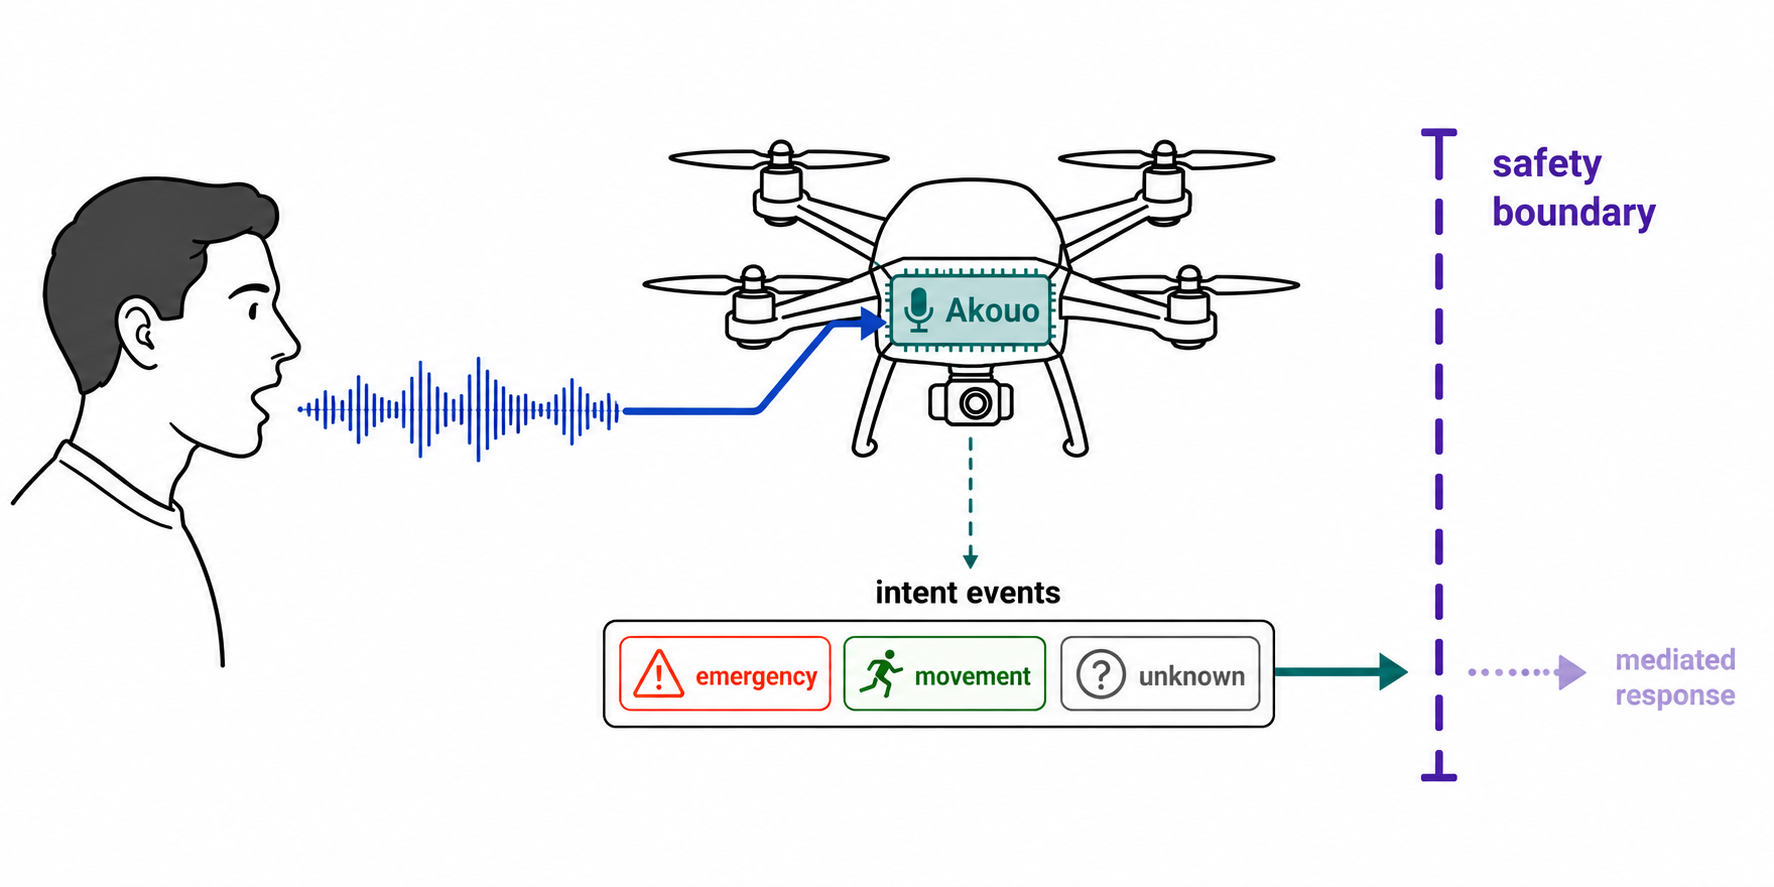
\includegraphics[width=\linewidth]{figures/figure1.png}
        \caption[Illustrative talk-to-the-drone scenario.]{Illustrative talk-to-the-drone scenario in which nearby speech provides a hands-free interaction channel while any UAV-facing response remains mediated by a safety-state boundary. This illustrative image was generated with ChatGPT from an author-provided prompt.}
        \label{fig:talk_to_drone_scenario}
        \Description{A nearby person speaks toward a rotor-noisy drone; the onboard Akouo layer reports an intent-state update that is mediated by a safety-state boundary before any response.}
    \end{minipage}
\end{figure}

Figure~\ref{fig:talk_to_drone_scenario} illustrates the interaction style this paper targets: nearby speech becomes an input to a UAV-side safety interaction layer rather than a direct replacement for the existing control stack.

Given the potential extent of applications of Unmanned Aerial Vehicles (UAVs), policymakers have been contemplating ensuring the deployment of these systems is bound by safety standards and regulations to potentially reduce unwarranted consequences. For example, Commission Implementing Regulation (EU) 2019/947 sets rules and procedures for the operation of unmanned aircraft, including operational requirements that depend on the risk category of the flight~\cite{eu2019uasops}. Such rules reflect a broader expectation that UAV deployments should consider operating conditions, risk mitigation, and fail-safe behavior. Most available UAVs on the market lack fault-detection systems, which can pose a safety risk. Soon, we expect regulators worldwide to establish safe operating conditions.

Speaking to a drone during an emergency is a natural reflex response because it aligns with how people react in such situations. It is an automatic and instinctive reaction to shout. For a nearby UAV, voice is especially useful because it is hands-free -- a person can express intent without reaching for a controller, opening a phone application, or relying on a network connection. It is also a real-time and immediate response to convey the dangerous situation the drone may get into. When the drone is very close to people or structures, or is about to collide with them, it should be able to understand voice commands, since speech is often the most natural way humans react in such situations.

However, the acoustic environment around a UAV is often highly challenging, with mainly propeller noise and other surrounding sounds making speech recognition highly difficult. This problem becomes much more severe for small UAVs or quadrotors, where the microphone will be very close to the propellers, causing strong self-noise. In addition, the noise spectrum changes with motor speed, distance, and drone motion. Prior work has shown that UAV speech interfaces are feasible in principle~\cite{oneata19_interspeech,oneata2021multimodal}, while studies on UAV noise indicate that operating conditions can significantly degrade voice-command recognition~\cite{miesikowska2021uavnoise,park2023uavvehicle}. The remaining systems gap is not only whether speech can be recognized near a drone, but whether short rotor-noisy speech can be converted locally, while the UAV is operating, into a constrained safety-state update before any vehicle-facing response is considered.

A straightforward response is to attach a conventional speech interface module to the drone -- transcribe the audio, parse the text, detect keywords, and map the recognized command directly to an action. This approach is attractive because it is simple and familiar, but it does not solve the safety-state boundary problem for small UAVs. Short rotor-noisy clips can make transcript-first parsing brittle; keyword or command classifiers can identify a label without defining how that label should be mediated before physical action; and direct mapping can turn recognition errors into immediate, unnecessary vehicle-facing actions.

% This paper introduces \emph{Akouo}, an onboard voice safety layer for small UAVs. Akouo listens for nearby speech and converts each short window of audio signal into a structured safety-state event  == "state of the intent for safe operations" before any action is considered. The event-state contract is deliberately small: movement represents an ordinary control-oriented request, emergency represents safety-critical speech, and unknown contains unsupported or uncertain audio. Akouo keeps this contract narrow so that ambiguous speech can be logged and contained instead of being forced into a flight command.

% intent?? three emergency "normal movement"  unknown

% safety-state event  == "state of the intent for safe operations"
% event-state = state of the event
%%%%%%%%%% Write again the above para here below
This paper introduces \emph{Akouo}, an onboard voice safety layer for small UAVs. In Akouo, an \emph{intent} is the speaker's communicative goal inferred from a short audio window. The recognizer does not output a flight command. Instead, it assigns each window to one of three intent states: \emph{emergency}, \emph{movement}, or \emph{unknown}. Emergency captures speech that should enter safety-critical handling, movement captures normal control-oriented speech, and unknown captures unsupported or uncertain audio. Akouo then reports this intent state with confidence and timing as an intent-state update for the safety-state boundary.
%%%%%%%%%%%%%%%%%%%%%%%%%%%%%%%%%%%%%%%%%%%%%%%%%%%%


This framing changes the evaluation question. Recognition accuracy still matters, but the system must also show why the intent-state mapping is needed, whether the recognizer can sustain the mapping under rotor noise, whether the embedded path can produce intent-state updates locally, and whether the safety-state boundary prevents unsupported speech from becoming an unintended action. We therefore evaluate Akouo against transcript-first, compact-classifier, and direct-mapping alternatives, not only as an isolated speech classifier.

\textbf{Our Approach.} Akouo follows three principles. First, the system should focus on the safety-relevant intent of speech, not on recovering every word. Second, the voice layer should run locally on the UAV whenever possible, so the onboard recognizer must fit the computation, memory, and operator constraints of the embedded processor. Third, speech should not directly trigger drone motion. The system must first produce an intent-state update, record confidence and timing, and pass the update through a safety-state boundary before any vehicle-facing response is allowed.

The prototype shows how this listening and recognition path can run close to the drone and produce intent-state updates for a boundary that logs and mediates possible actions.

Akouo is not a replacement for collision avoidance, geofencing, emergency landing, or manual override. Instead, it adds a way for nearby people to express speech-based intent, which the UAV can record and check before any action is considered.

%%%The evaluation is organized around the same layers. Offline recognition tests evaluate whether the system can separate movement, emergency, and unknown speech under rotor-noisy conditions. Board-level tests evaluate whether the local hardware can capture audio, run the recognizer, and report events reliably. Control-side tests are needed to evaluate how those events are ignored, held, escalated, or forwarded by the bridge. We keep these claims separate because recognition accuracy alone does not prove a safe UAV interaction, and a working board pipeline does not prove readiness for live flight.

%%%********* PLEASE REWITE ABOVE TWO PARAS TO MAKE IT EASY TO UNDERSTAND STORY .... BECAUSE THE READER IN THE BEGINNING WILL NOT HAVE ANY IDEA OF THE SPECIFIC WORDS YOU USE!!! ************ Please 
%%%%%%%%%%%%%%%%%%%%%%%%%%%%%%%%%%%%%%%%%%%%%
% contract => construct: Synonyms
% STRONGEST
% build up
% compose
% create
% design
% erect
% establish
% fashion
% forge
% form
% formulate
% found
% manufacture
% organize
% produce
% put up
% set up
% shape
% STRONG
% compound
% constitute
% elevate
% engineer
% envision
% fabricate
% frame
% imagine
% invent
% make
% prefab
% raise
% rear
% WEAK
% cobble up
% cook up
% dream up
% fudge together
% hammer out
% hoke up
% put out
% put together
% throw together
% throw up
% trump up
% uprear
% whip up
%%%%%%%%%%%%%%%%%%%%


This paper makes four contributions:
\begin{itemize}
\item \textbf{A speech-admission abstraction for UAV safety interaction.} We identify the missing systems layer between speech recognition and UAV action: nearby speech should not enter a physical control stack as text, keywords, or direct commands. \sys{} treats speech as evidence that must first be admitted through a safety-state boundary.
\item \textbf{A constrained intent-state interface for noisy human input.} We define a small event vocabulary whose semantics are tied to safe admission rather than command execution. Emergency, movement, and unknown are not merely classifier labels: they specify whether speech should enter safety-critical handling, remain pending for authority and vehicle-state checks, or be contained as unsupported audio.
\item \textbf{An onboard rotor-noisy recognizer for that interface.} We build the intent-state source around the actual operating condition: one-second nearby speech mixed with rotor self-noise, local feature extraction, and embedded-compatible inference. The recognizer uses clean/noisy alignment and a compact Branchformer-style temporal encoder to report intent state, confidence, and timing locally, without issuing vehicle-facing commands.
\item \textbf{Evidence organized around the failure modes of naive designs.} We evaluate \sys{} against the alternatives implied by the abstraction: transcript-first ASR with deterministic parsing, compact speech-command model-family baselines under the same three-intent rotor-noisy task, direct-mapping and no-unknown action-pressure simulations, embedded capture-to-inference timing, and participant-level onboard recognition.
\end{itemize}

The rest of the paper is organized as follows. Section~\ref{sec:related} reviews related work in UAV speech interfaces, embedded speech recognition, and UAV safety mechanisms. Section~\ref{sec:motivation} motivates constrained intent states under drone self-noise. Section~\ref{sec:system} presents the system architecture and intent-state mapping. Section~\ref{sec:recognizer} describes the recognizer design. Section~\ref{sec:prototype} presents the prototype and safety-state boundary interface. Section~\ref{sec:evaluation} evaluates the system components and contrasts Akouo with common speech-interface alternatives. Section~\ref{sec:discussion} discusses limitations and extensions, and Section~\ref{sec:conclusion} concludes.
